\newpage
\subsubsection{DJI Phantom 4}
\begin{wrapfigure}{r}{0.3\textwidth}
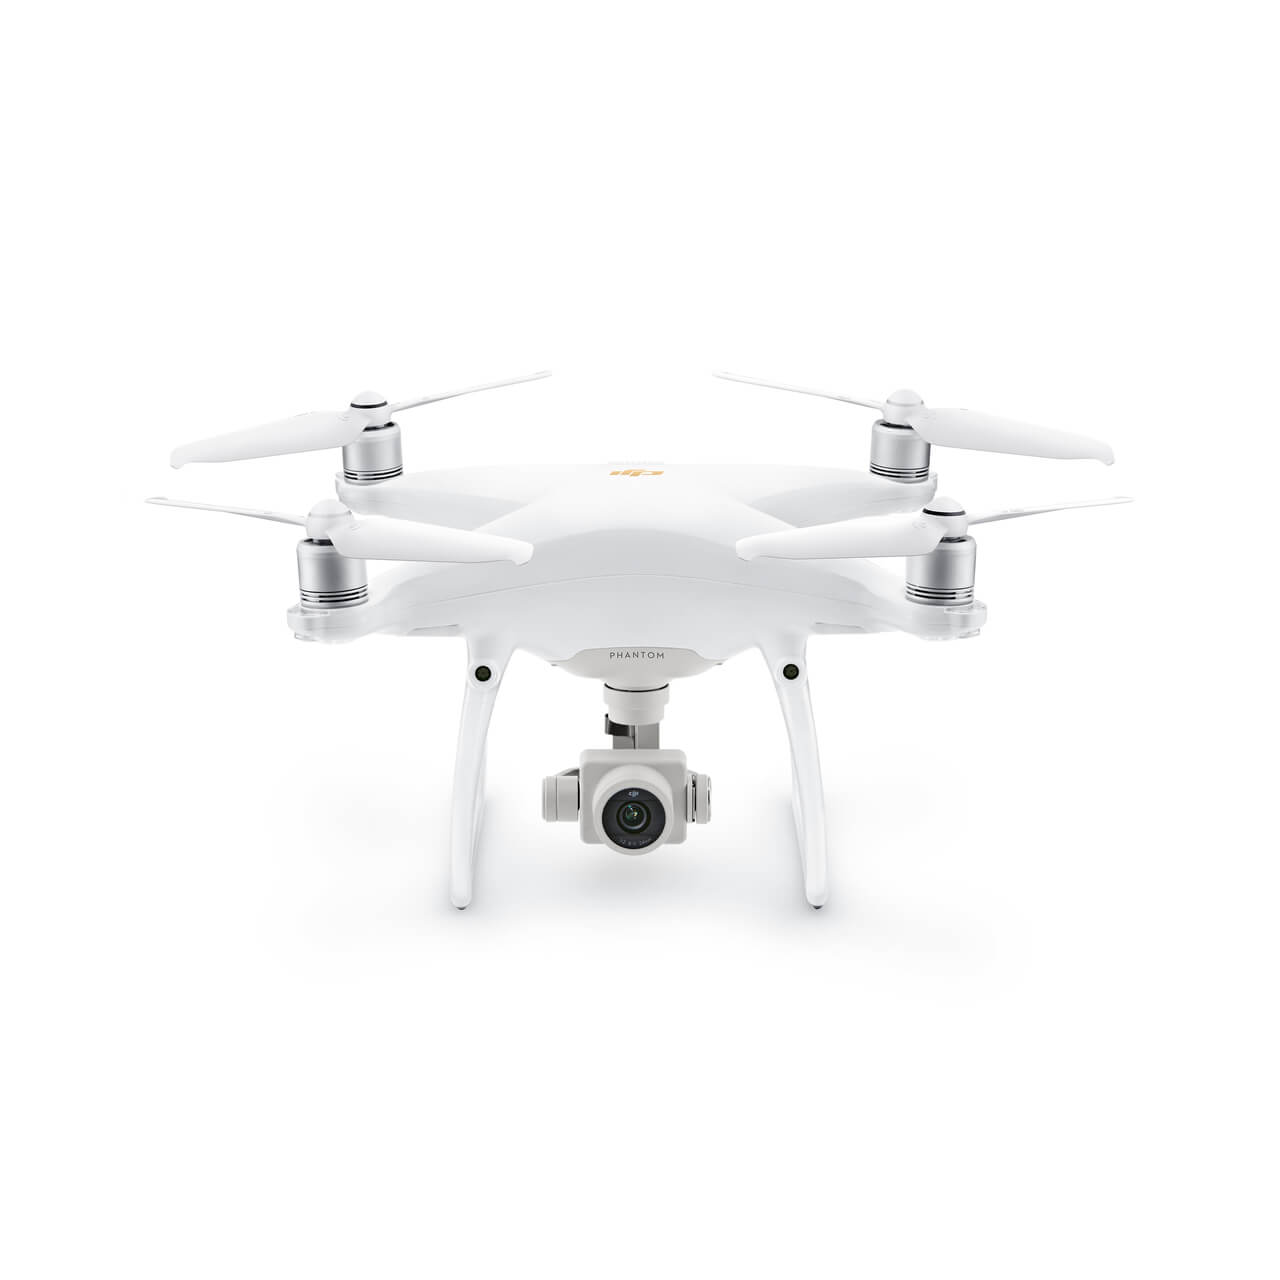
\includegraphics[width=1\linewidth]{uav/models/41_phantom4.jpg}
\caption{Phantom 4}
\end{wrapfigure}
The Phantom 4 \cite{phantom4} was one of DJI's flagship drones. While there have been several variants of this popular drone, like the V2.0 Pro, they are identical to our requirements.

\paragraph{Payload capacity}\mbox{Score: 1.0} \\
While DJI only notes payload capacity on the Matrice 300 Series, the payload capacity of the Phantom 4 is generally considered to be 500 grams. This has been tested by multiple frequent users of the drone. \cite{phantompilots} 

\paragraph{Mounting clearance}\mbox{Score: 1.5} \\
The Phantom 4 is one of the bigger drones. Due to it's popularity, it has several third party mounting solutions that one can buy \cite{polarpro} or build themselves \cite{thingiverse}. One could easily use these mounting solutions to mount sensors or water collectors.

\paragraph{Navigation/Routing}\mbox{Score: 1.5} \\
One can plan routes for the Phantom 4 using the well established DJI Go 4 app \cite{djigo} available on iOS and Android. There is also the excellent DroneExpert search and rescue flight app available on iOS which is designed to pre-program an ideal flight route. \cite{desar}

\paragraph{Flight time}\mbox{Score: 1.3} \\
The flight time of the Phantom 4 is 22 minutes, passing the minimum required flight time.

\paragraph{Range}\mbox{Score: 1.5} \\
The maximum radio range is 5.0km, well over the minimum required range. This also includes image transmission.

\paragraph{Waterproof}\mbox{Score: 1.0} \\
The Phantom 4 is not waterproof by default, but there are wetsuits available which makes the drone dust-tight and immersible up to 1 meter in water, basically creating it IP67 proof. \cite{phantomrain}

\paragraph{Landing in water}\mbox{Score: 0.8} \\
While the Phantom 4 does not have a water landing gear by default, there are commercial kits one can buy to make the drone able to land on water. \cite{buylanding} One could also create their own water landing gear. \cite{diylanding}

\paragraph{Maneuverability}\mbox{Score: 1.4} \\
Because the Phantom 4 is a somewhat bigger drone, it can fly horizontally a maximum of 10m/s. DJI has made sure that even under load the drone is stable.

\paragraph{Total score:}\mbox{4.9} \\
The Phantom 4 seems like a stable option given it's price on the used market and it's popularity in the drone community. DJI's experience in creating drones makes that the drone is less likely to have deal breaking bugs. Replacement parts are also readily available. The downside to this drone is primarily that you will be doing a new project with older hardware that isn't supported by DJI anymore.